\documentclass{article}

% Language setting
% Replace `english' with e.g. `spanish' to change the document language
\usepackage[english]{babel}
\usepackage{mathptmx}

% Set page size and margins
% Replace `letterpaper' with`a4paper' for UK/EU standard size

% Useful packages
\usepackage{amsmath}
\usepackage{graphicx}
\usepackage[colorlinks=true, allcolors=blue]{hyperref}

\usepackage{float}


\title{Projet Long}
\author{Ait benali Faycal
Bouchachia Ayoub, Boucherir Mohamed Zineddine}

\begin{document}
\maketitle
  





\newpage
\hypersetup{linkcolor=black}
\setcounter{tocdepth}{1}
\tableofcontents
\addtocontents{toc}{~\hfill\textbf{Page}\par}


\newpage




\section{Introduction générale}


\paragraph{}Depuis les deux dernières décennies,  internet est devenu un outil incontournable de recrutement.Les méthodes de recherche et les relations avec les candidats ont profondément changé. Le e-recrutement se structure et évolue.
En effet , ce média puissant offre à l’entreprise, quelle que soit sa taille, un potentiel important de candidats qui apportent au recruteur : ciblage pertinent, rapidité, coûts maitrisés et ouverture sur le monde, pour des recrutements ponctuels, récurrents ou de masse tant en France qu’à l’international. De nombreux sites emploi sont, aujourd’hui, la première source de CV qualifiés , ainsi le é-recrutement est devenu un des services en ligne les plus populaires pour les demandeurs d'emploi ainsi que pour les employeurs. 
Néanmoins, le processus de recrutement et de recherche d'emploi n'est pas facile, notamment en ce qui concerne la recherche de profils et de talents, car de nombreuses approches se limitent actuellement à la recherche par mots-clé, qui n'est plus efficace lorsque la taille des données devient énorme. 

\paragraph{}Dans ce projet, nous présentons SEEKJOBS un système de recommandation d'offre d'emploi  basé sur les méthodes d'apprentissage automatique et du traitement du langage naturel. Ce système permet au recruteur de trouver les meilleurs candidats à un emploi et aide aussi les chercheurs d'emploi à trouver les emplois appropriés à leurs profiles les présentés dans les CVs. 
La recommandation est basé sur un modèle de classifcation des textes et le calcul de similarités entre l'offre d'emploi et les CVs des candidats. 
Dans ce rapport , nous présenterons un aperçu des données utilisées, leur collections et les différentes traitements faites sur le corpus d'entraînement. l'extraction d'informations à partir des CVs, les démarches de la formation d'un modèle de classification et le modèle de similarité sont aussi présentés dans ce chapitre. 
En fin ,  une conclusion contenant le bilan et les différentes perspectives pour améliorer ce travail. 


\section{Collecte des données}
Nous avons utilisé les techniques du web scrapping pour collecter les données du site Indeed.
\subsection{web scrapping}
\paragraph{}C'est une technique utilisée pour extraire des données des sites web. Il s'agit d'un processus automatisé dans lequel une application traite le code HTML d'une page web afin d'extraire des
données
Les étapes de la collection des CVs
\begin{enumerate}
    \item L'examination de l'URL et la page contenant les résultats de la recherche.
    \item L'extraction des liens des CVs.
    \item L'extraction des données des CVs.
    \item La segmentation des CVs en blocs.
    \item Le stockage des données collectées dans un fichier "json".
    
    \begin{figure}[H]
  	\centering
    	  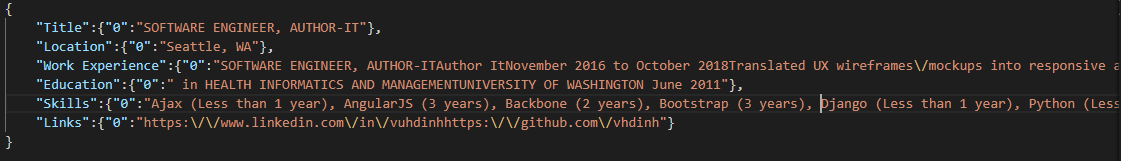
\includegraphics[width=1.0\textwidth]{Figures/cvseg.PNG}
  		\caption{Un cv segmenté (Corpus de CV)}
  	\label{json}
\end{figure}

\end{enumerate}


\section{L'architecture générale}
L'architecture générale de notre système de recommandations est donnée par la figure
\begin{figure}[H]
  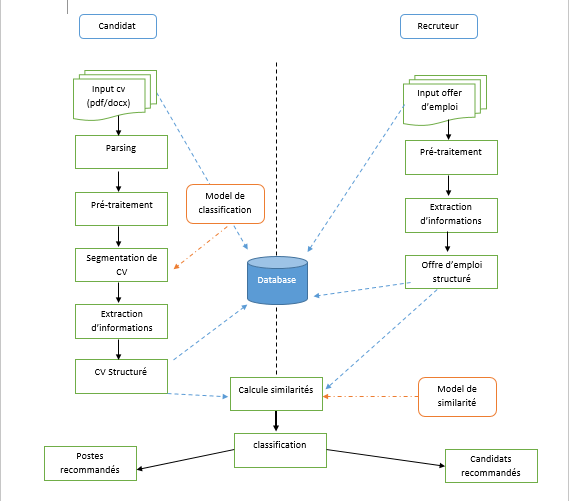
\includegraphics[width=\linewidth ]{Figures/architecture.png}
  \caption{\label{arch}Architecture de SEEKJOBS}

\end{figure}	


 
\section{Ségmentation du CV }
\paragraph{}Pour la segmentation des CVs nous avons utilisé un classificateur de texte pour identifier la classe des différents blocs (skills, education, work experience). Nous avons utilisé les CVs collectés pour l'entrainement du modèle. 
\begin{figure}[H]
  \includegraphics[width=\linewidth ]{Figures/distribution_des_données_selon_les_classes.png}
  \caption{\label{arch}distribution des données selon les classes}
\end{figure}

\subsection{Pré-traitement }
\paragraph{}Les données textuelles brutes exprimées en langage naturel ne sont pas utilisables directement
par la machine. 
\paragraph{}L'étape de prétraitement a donc a pour objectif de préparer le texte pour la
phase d'apprentissage. Techniquement, c'est l'étape de nettoyage du texte (éliminer les termes
et caractères non signicatifs), l'extraction des occurrences des termes définissant les segments
et le calcul des fréquences de ces derniers.

\paragraph{} Ensuite, tous les mots sont convertis en minuscules puis traités à l'aide de Porter Stemmer du package NLTK. Le but est de diminuer le nombre de mots flexibles apparaissant dans les CVs. Cela permet de réduire la taille du vocabulaire et d'améliorer le volume de l'espace des fonctions dans le corpus.

\subsection{Apprentissage}

\paragraph{}Lors de la construction du modèle, nous pouvons choisir parmi une large gamme d'algorithmes
de classication. Nous avons testé quatres algorithmes diérents : KNN, multinomial naïf Bayes,
linéaire SVC.
\paragraph{}Avant de comparer les performances des différents algorithmes de classification, nous nous
sommes basés sur des mesures de statistiques communes tels que la précision et le rappel.
Après avoir testé les algorithmes, les expérimentation ont montré que l'algorithme de du classificateur naif de bayes est simple et facile à deployer par rapport aux autres.

\subsubsection{classifieur Naïve Bayes}
 \paragraph{} Cette méthode se base sur le théorème de Bayes qui permet de calculer les probabilités conditionnelles. 
 
 Dans le cas de la classification du texte, la méthode Naïve Bayes est utilisée comme suit : on cherche la classification qui maximise la probabilité d'observer les mots du document. Lors de la phase d'entraînement, le classifieur calcule les probabilités qu'un nouveau document appartient à telle catégorie à partir de la proportion des documents d'entraînement appartenant à cette catégorie. 
 Il calcule aussi la probabilité qu'un mot donné soit présent dans un texte, sachant que ce texte appartient à une telle classe. Quand un nouveau document doit être classé, on calcule les probabilités qu'il appartient à chacune des classes à l'aide de la règle de Bayes et on prend la classe la plus probable.



Soit le jeu de données $D$ (corpus) composé de $n$ paires $(x,c)$, avec $x$ un document qui contient un ensemble de mots $w$ et $c$ la classe auquel ce texte appartient parmi $q$ classes possibles :
\newline

\begin{center}
$D=\{(x_1,c_1),(x_2,c_2),...,(x_n,c_n)\}  \forall (x_i,c_i)_{1 \leq i \leq n}, c_i \in \{y_1,y_2,...,y_q\}, x_i=\{w_1,w_2,...,w_{di}\}$

\end{center}



Le modèle Naïve Bayes modélise la probabilité jointe d'un texte $x$ et de sa catégorie $y$ $P(X=x , Y=y)$. Par définition  :
\newline

\begin{center}
$P(X=x,Y=y)=P(Y=y)P(X=x|Y=y)$
\end{center}

Prenons comme hypothèse que mots dépendent seulement de la classe et il sont indépendants entre eux, on peut réécrire $P(X=x , Y=y)$ comme le produit des probabilités conditionnelles des mots.
\newline

\begin{center}
$P(X=x|Y=y)=P(X=[w_1,w_2,...,w_d]|Y=y)=\prod_{k=1}^d P(W=w_k|Y=y)$
\end{center}


Ainsi, on obtient :
\newline

\begin{center}
$P(X=x,Y=y)=P(Y=y)\prod_{k=1}^d P(W=w_k|Y=y)$
\end{center}


La classe d'une nouvelle observation z est déterminée selon la règle décision suivante :
\newline

\begin{center}
$\hat{y} = argmax_{j \in \{1,2,...,q\}}\{P(Y=y_j|X=z)\}$
\end{center}


En appliquant le théorème de Bayess :
\newline

\begin{center}
$\hat{y} = argmax_{j \in \{1,2,...,q\}}\{\frac{P(X=z|Y=y_j)P(Y=y_j)}{P(X=z)}\}$
\end{center}


Comme le dénominateur, $P(X=z)$, ne dépend pas de Y, sa valeur est constante et minimiser l'expression ci-dessus revient à maximiser :
\newline


\begin{center}
\item $\hat{y} = argmax_{j \in \{1,2,...,q\}}\{P(X=z|Y=y_j)P(Y=y_j)\}$
\item $\hat{y} = argmax_{j \in \{1,2,...,q\}}\{P(Y=y_j)\prod_{k=1}^{d_z} P(W=w_k|Y=y_j)\}$
\end{center}



Si on pose $P(Y=y_j)=g(y_j)$ et $P(W=w_k|Y=y_j)=g_k(w_k|y_j)$ , le modèle Naïve Bayes s'écrit comme suit :
\newline

\begin{center}
$\hat{y} = argmax_{j \in \{1,2,...,q\}}\{g(y_j)\prod_{k=1}^{d_z} g_k(w_k|y_j)\}$
\end{center}

Où $g(y_j)$ et $g_k(w_k|y_j)$ sont des paramètres à estimer.
\newline

On estime la probabilité apriori d'observer la classe y en mesurant sa fréquence relative dans D (le nombre de documents qui ont la classe $y_j$ comme catégorie sur le nombre total de documents):
\newline

\begin{center}
$g(y_j)=\frac{\sum_{i=1}^n (y_j=y_i)}{n}$
\end{center}


On estime la probabilité d'observer le mot $w_k$ conditionnellement à la classe $y_j$ en calculant le rapport entre le nombre de fois que $w_k$ apparaît dans les documents de la catégorie $y_j$ ,et le nombre de mots total dans les documents de la catégorie $y_j$:
\newline

\begin{center}
$g(w_k|y_j)_k=\frac{\sum_{i=1}^n [(y_j=y_i)\sum_{r=1}^{d_i}(w_k=w_r)]}{\sum_{i=1}^n [(y_j=y_i) d_i ] }$
\end{center}
\begin{figure}[H]
  \centering
      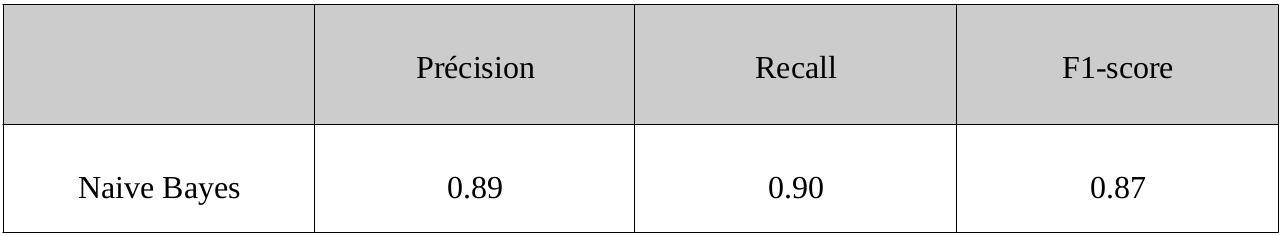
\includegraphics[width=1.0\textwidth]{Figures/table.PNG}
    \caption{la performance des modèles de classi}
  \label{json}
\end{figure}

\section{Diffcultés retrouvées}
\paragraph{}Durant la réalisation , nous avons retrouvé quelques difficultés techniques (liées au materiel) nottament le stockage , en effet , nous n'avons pas pu faire l'apprentissage , sur toutes les données qu'on a collecté , comme elle ont une taille très grande , ce qui nous a poussé à diminuer la taille des données pour pouvoir avancer 
\section{Fonctionnalité non encore implémentées}
\paragraph{}A cette étape, nous avons réaliser une partie importante du projet , mais il reste encore des taches à faire, en l'occurence la plateforme Web.
En plus , il reste la partie de calcul de similarité entre une offre d'emploi et un CV, ce qui nous permet de réaliser la recommandation.


\section{Outils}
\paragraph{}En ce qui concerne les outils et langage de programmation que nous avons jugé utiles pour notre réalisation nous avons utilisé pour réaliser le porjet  : Python, Selenium, BeautifulSoup, NLTK, scikit-learn et django, et concernant la création de design de site web du côté client nous avons opté pour Bootstrap . 


\newpage
\section{Conclusion}

\paragraph{}
Nous nous sommes intéressés dans ce travail à concevoir et implémenter un système de recommandation d'emploi qui facilite le processus de recrutement et de la recherche d'emploi. Nous avons choisi de travailler sur les données d'un seul domaine de travaille.

\paragraph{}Nous avons choisi une approche basée sur le contenu des CVs et des offres d'emploi pour concevoir notre système.

\paragraph{} Nous avons utilisé les différentes techniques du TALN afin d'extraire les informations pertinentes à partir des CVs et les offres d'emploi tels que les compétences et la formation.

\paragraph{} Un modèle de classification de textes a été entrainé  qui permet de mieux segmenter le CV selon la catégorie des informations qu'il présente.


\paragraph{} il nous reste l'implémentation d'un modèle de similarité pour permettre de faire la correspondance entre les CVs et les offres d'emploi, et la plateforme web afin de mettre en œuvre notre système de recommandation.

\paragraph{}Nous citons comme perspectives les questions suivantes qui pourraient améliorer notre système :
\begin{itemize}
	\item ajouter un questionnaire personnalisé selon le CV, pour évaluer les compétences du candidat.
	\item Généraliser notre modèle pour travailler dans un contexte multilingue et trouver un benchmark  permettant de meilleurs tests.
	
	\item Utiliser l'approche hybride pour améliorer les recommandations et tester d'autres modèles d'apprentissage automatique.
	
	\item Automatiser l'ajout de nouveaux domaines de travaille et l'entrainement des modèles de classification et similarité selon les données de ce domaine.
\end{itemize}


\end{document}